% ****** Start of file apssamp.tex ******
%
%   This file is part of the APS files in the REVTeX 4.1 distribution.
%   Version 4.1r of REVTeX, August 2010
%
%   Copyright (c) 2009, 2010 The American Physical Society.
%
%   See the REVTeX 4 README file for restrictions and more information.
%
% TeX'ing this file requires that you have AMS-LaTeX 2.0 installed
% as well as the rest of the prerequisites for REVTeX 4.1
%
% See the REVTeX 4 README file
% It also requires running BibTeX. The commands are as follows:
%
%  1)  latex apssamp.tex
%  2)  bibtex apssamp
%  3)  latex apssamp.tex
%  4)  latex apssamp.tex
%
\documentclass[%
 reprint,
%superscriptaddress,
%groupedaddress,
%unsortedaddress,
%runinaddress,
%frontmatterverbose, 
%preprint,
%showpacs,preprintnumbers,
%nofootinbib,
%nobibnotes,
%bibnotes,
 amsmath,amssymb,
 aps,
%pra,
%prb,
%rmp,
%prstab,
%prstper,
%floatfix,
10.5pt,
]{revtex4-1}

\usepackage{graphicx}% Include figure files
\usepackage{subfigure}
\usepackage{multirow}
\usepackage{array}
\usepackage{dcolumn}% Align table columns on decimal point
\usepackage{bm}% bold math
%\usepackage{hyperref}% add hypertext capabilities
%\usepackage[mathlines]{lineno}% Enable numbering of text and display math
%\linenumbers\relax % Commence numbering lines

%\usepackage[showframe,%Uncomment any one of the following lines to test 
%%scale=0.7, marginratio={1:1, 2:3}, ignoreall,% default settings
%%text={7in,10in},centering,
%%margin=1.5in,
%%total={6.5in,8.75in}, top=1.2in, left=0.9in, includefoot,
%%height=10in,a5paper,hmargin={3cm,0.8in},
%]{geometry}

\usepackage{xeCJK}
\setCJKmainfont[ItalicFont={KaiTi}, BoldFont={KaiTi}]{KaiTi}
\usepackage{textcomp}
\usepackage{chemfig}
\usepackage[version=4]{mhchem}
\usepackage{fontspec}
\usepackage{listings}
\usepackage{xcolor}
\usepackage{xcolor} % 定制颜色
\definecolor{mygreen}{rgb}{0,0.6,0}
\definecolor{mygray}{rgb}{0.5,0.5,0.5}
\definecolor{mymauve}{rgb}{0.58,0,0.82}
\lstset{
backgroundcolor=\color{white},      % choose the background color
basicstyle=\footnotesize\ttfamily,  % size of fonts used for the code
columns=fullflexible,
tabsize=4,
breaklines=true,               % automatic line breaking only at whitespace
captionpos=b,                  % sets the caption-position to bottom
commentstyle=\color{mygreen},  % comment style
escapeinside={\%*}{*)},        % if you want to add LaTeX within your code
keywordstyle=\color{blue},     % keyword style
stringstyle=\color{mymauve}\ttfamily,  % string literal style
frame=single,
rulesepcolor=\color{red!20!green!20!blue!20},
% identifierstyle=\color{red},
language=Mathematica,
}

\usepackage[normalem]{ulem}

\newcommand{\chuhao}{\fontsize{42pt}{44.9pt}\selectfont}    % 初号, 1.5倍行距
\newcommand{\xiaochu}{\fontsize{30pt}{40pt}\selectfont}    % 小初, 1.5倍行距
\newcommand{\yihao}{\fontsize{26pt}{36pt}\selectfont}    % 一号, 1.4倍行距
\newcommand{\erhao}{\fontsize{22pt}{28pt}\selectfont}    % 二号, 1.25倍行距
\newcommand{\xiaoer}{\fontsize{18pt}{18pt}\selectfont}    % 小二, 单倍行距
\newcommand{\sanhao}{\fontsize{16pt}{24pt}\selectfont}    % 三号, 1.5倍行距
\newcommand{\xiaosan}{\fontsize{15pt}{22pt}\selectfont}    % 小三, 1.5倍行距
\newcommand{\sihao}{\fontsize{14pt}{21pt}\selectfont}    % 四号, 1.5倍行距
\newcommand{\sihaox}{\fontsize{14pt}{28pt}\selectfont}    % 四号, 1.5倍行距
\newcommand{\banxiaosi}{\fontsize{13pt}{19.5pt}\selectfont}    % 半小四, 1.5倍行距
\newcommand{\xiaosix}{\fontsize{12pt}{24pt}\selectfont} 	% 小四, 1.5倍行距
\newcommand{\xiaosi}{\fontsize{12pt}{18pt}\selectfont}     
\newcommand{\dawuhao}{\fontsize{11pt}{11pt}\selectfont}    % 大五号, 单倍行距
\newcommand{\wuhao}{\fontsize{10.5pt}{10.5pt}\selectfont}    % 五号, 单倍行距
\newcommand{\xiaowu}{\fontsize{9pt}{9pt}\selectfont}    % 五号, 单倍行距

%\usepackage[fntef]{ctexcap}
%\CTEXsetup[number={\chinese{section}、},format={\Large\bfseries}]{section}
\setCJKfamilyfont{fangsong}{FangSong}                      %仿宋2312 fs  
\newcommand{\fangsong}{\CJKfamily{fangsong}}  

\usepackage{wrapfig}
\usepackage{fancyhdr}
\usepackage{fancybox}   






\newcommand{\bra}[1]{\langle #1 |}
\newcommand{\ket}[1]{| #1 \rangle}
\newcommand{\bracket}[2]{\langle #1 | #2 \rangle}
\newcommand{\bracketl}[3]{\langle #1 | #2 | #3 \rangle}
\newcommand{\func}{\mathrm \,}
\newcommand{\define}[2]{
	\begin{definition}
	\begin{description}
	\item[#1]
	#2
	\end{description}
	\end{definition}
}

\newcommand{\sch}{Schr\"odinger}
\newcommand{\grad}{\nabla}
\newcommand{\ueq}{\neq}
\newcommand{\celsius}{\ensuremath{^\circ\hspace{-0.09em}\mathrm{C}}}
\newcommand{\unit}[2]{$#1 \, \mathrm{#2}$}

\begin{document}

%\preprint{APS/123-QED}

\title{Measurement of heat of combustion of stearyl alcohol}% Force line breaks with \\
%\thanks{A footnote to the article title}% give thanks

\author{Rui Li}
 %\altaffiliation[Also at ]{Physics Department, XYZ University.}%Lines break automatically or can be forced with \\
%\author{Second Author}%
%\email{3160102098@zju.edu.cn}
\affiliation{%
 Qiushi science class (chemistry)\\
 Chu Kochen Honor College
}%

%\collaboration{MUSO Collaboration}%\noaffiliation

%\author{Zong Wei Huang}
% \homepage{http://www.Second.institution.edu/~Charlie.Author}
%\affiliation{
% Second institution and/or address\\
% This line break forced% with \\
%}%
%\affiliation{
%Qiushi science class (chemistry)\\
% Chu Kochen Honor College
%}%
%\author{Delta Author}
%\affiliation{%
% Authors' institution and/or address\\
% This line break forced with \textbackslash\textbackslash
%}%

%\collaboration{CLEO Collaboration}%\noaffiliation

%\date{\today}% It is always \today, today,
             %  but any date may be explicitly specified

\begin{abstract}
Heat of combustion of stearyl alcohol is measured using bomb calorimeter, the process of which is well simulated using one-dimension model, indicating better way to correct the change of the temperature resulted from the combustion.
\begin{description}
\item[Keywords]
heat of combustion, bomb calorimeter, simulation
\end{description}
\end{abstract}
\bibliographystyle{unsrt}
%\pacs{Valid PACS appear here}% PACS, the Physics and Astronomy
                             % Classification Scheme.
%\keywords{Suggested keywords}%Use showkeys class option if keyword
                              %display desired
\maketitle

\tableofcontents

\section{Introduction}
Heat of combustion is a fundamental parameter when giving quantitative analysis on the energy of a substance. It represents the difference of enthalpy of two states: the initial state for the matter, the end state for the stable products after chemical reaction. With this many other data can be deduced or estimated, which provide essential information for researches.

Combustion usually involves forming of gas, which challenges the firmness of the container, while an adiabatic environment is also vital for measuring heat explicitly. A bomb calorimeter is designed to satisfy these requirements, which consists of a small cup to contain the sample, oxygen of high pressure to ensure complete reaction, a stainless steel bomb, water, a stirrer, a thermometer, the dewar or insulating container (to prevent heat flow from the calorimeter to the surroundings) and ignition circuit connected to the bomb. After the sample reacts completely, the heat produced is gradually absorbed by the surrounding water, and the change of temperature is detected, then the Heat of combustion can be derived. 

Nonetheless, the calorimeter still cannot eliminate heat exchanges with environment, while stirring also provides extra heat. Thus a correction of temperature is applied, which involves drawing two lines from initial and final temperature curves. Difference exists at different time between these two lines, and the time when the temperature reaches the median is chosen to calculate the corrected change of temperature, thus the loss of heat is compensated, while extra heat introduced by stirring is also reduced from the result.

\section{Devices and Procedures}
A bomb calorimeter is prepared, containing certain amounts of samples and 1.5 MPa of oxygen compressed in the steel bomb, with precise amount of 3,000 mL of water added to keep the heat capacity of the whole apparatus constant. Copper string is used to ignite the sample.The temerature is measured by Pt-1000 thermometer and recorded by SunyLAB200 Data Recorder. The temperature curve keeps straight for at least 3 minutes before ignition, and for at least 5 minutes before finishing the recording. The water is refreshed after each round. Pure benzoic acid is utilized to measure the exact heat capacity of the apparatus, and the heat of combustion of stearyl alcohol is then measured. The data is analyzed and plotted using \emph{Mathematica}.


\section{Results and Analysis}
Correction of the change of temperature is realized by codes:
\begin{lstlisting}
ReynoldsTempCorrect[data_] := Module[{median, center, range},timing
  median = (Max[#] + Min[#])/2 &[data];
  center = 
   First@First@
     Position[data, 
      First@Sort[data, Abs[#1 - median] < Abs[#2 - median] &]];
  range = 
   Normal[LinearModelFit[#, {1, x}, x]] & /@ {Take[data, 100], 
      Take[data, -100]} /. x -> center;
  Abs[Subtract @@ range]
  ]
\end{lstlisting}

The data recorded and calculated are shown in Table.\ref{result}. Curves plotted are shown in Fig.\ref{BA} and Fig.\ref{R}. The comparison between the result from the experiment and from the reference show that the data is fairly reliable ($1.167 \times 10^4$ kJ/mol/K \emph{v.s.} $11820. \pm 4$ kJ/mol/K\cite{freedman1989heats}), thanks to the relatively adiabatic environment provided by the bomb calorimeter. Deviations may arise from the incompleteness of the reaction, the insensitivity of the thermometer which affects the process of correction of temperature, and choice of time in the correction process. Deviation from standard room temperature is slightly to blame for the error, which affects the heat capacity of the system.

\begin{table}
\centering
\caption{The result of the experiment, where BA stands for benzoic acid, and R for stearyl alcohol.}
\begin{tabular}{c|cc|ccc}\hline
 & \multicolumn{5}{c}{Test Group} \\\hline
Data &  R,1 & R,2 & BA,1 & BA,2 & BA,3 \\\hline
$m_\text{sample}$/g & 0.4235 & 0.6320 & 0.7840 & 0.8406 & 0.9043 \\
$\Delta m_\text{Cu}$/g & 0.0220 & 0.0202 & 0.0091 & 0.0150 & 0.0164  \\
$\Delta T/\celsius$ & 1.296 & 1.881 & 1.452 & 1.564 & 1.662 \\
$C_V$/(kJ/mol/K) & \multicolumn{2}{c|}{N/A} & 14.30 & 14.24 & 14.43 \\
$\bar{C_V}$/(kJ/mol/K) & \multicolumn{2}{c|}{N/A} & \multicolumn{3}{c}{14.32} \\
$Q$/($10^4$ kJ/mol) & -1.182 & -1.151 & \multicolumn{3}{c}{N/A} \\
$\bar{Q}$/($10^4$ kJ/mol) & \multicolumn{2}{c|}{-1.167} & \multicolumn{3}{c}{N/A}\\\hline
\end{tabular}
\label{result}
\end{table}

\begin{figure}
\centering
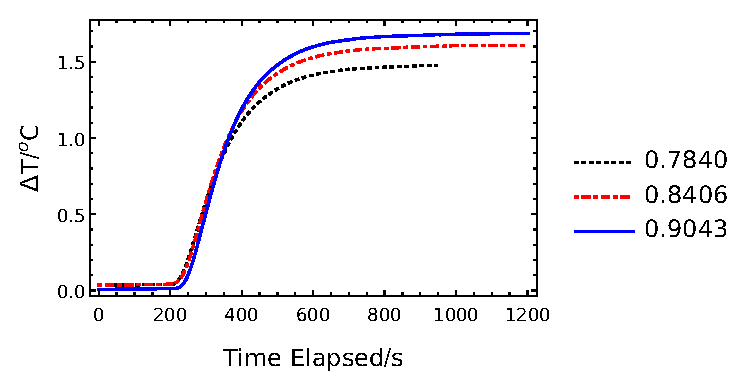
\includegraphics[width=0.4\textwidth]{figures/BATemp.eps}
\caption{The $T\,-\,t$ curves for combustion of benzoic acid. The legends stand for the mass of the sample.}
\label{BA}
\end{figure}

\begin{figure}
\centering
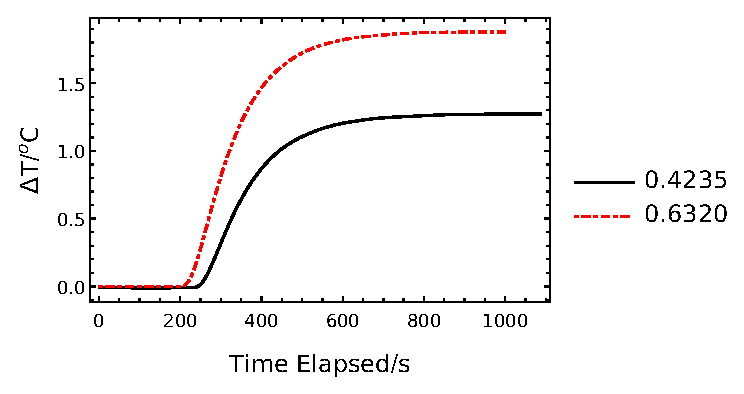
\includegraphics[width=0.4\textwidth]{figures/18olTemp.eps}
\caption{The $T\,-\,t$ curves for combustion of stearyl alcohol. The legends stand for the mass of the sample.}
\label{R}
\end{figure}

Simple one-dimension model of such an experiment is fabricated and programmed in \emph{julia}, which fits the curves from the experiment nicely, as revealed in Fig.\ref{expsim}. The chamber is set middle of the box of 30 cells, and heat flow is simulated according to the formula

\begin{equation}
\begin{cases}
\frac{\Delta q}{\Delta t} \sim D_f \frac{T(x+\Delta x)+T(x-\Delta x)-2T(x)}{2\Delta x}\\
\Delta  T(x) \sim \frac{\Delta q /\Delta t}{C_V}\Delta t.
\end{cases}
\end{equation}

It shows that the model is verified, deviation from experimental curve of which is attributed to the absense of stirring process that involves much complicated algorithms to simulate. Fig.\ref{combustbox}
 partly reveals the whole process of the heat flow from the chamber to the very edges of the system. A certain amount of time needs to be spared for the whole system to `react' to the sudden heating from the chamber and for the heat to flow over. The relatively slow heat conduction between the chamber and the surrounding water is also simulated, which is also responsible for the delay of the heat flow. 

\begin{figure}
\centering
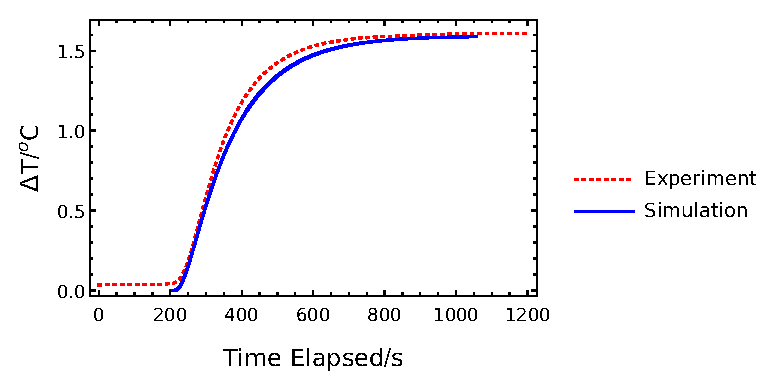
\includegraphics[width=0.4\textwidth]{figures/simuvsexp.eps}
\caption{The curves for experiment \emph{v.s.} simulation}
\label{expsim}
\end{figure}

\begin{figure}
\centering
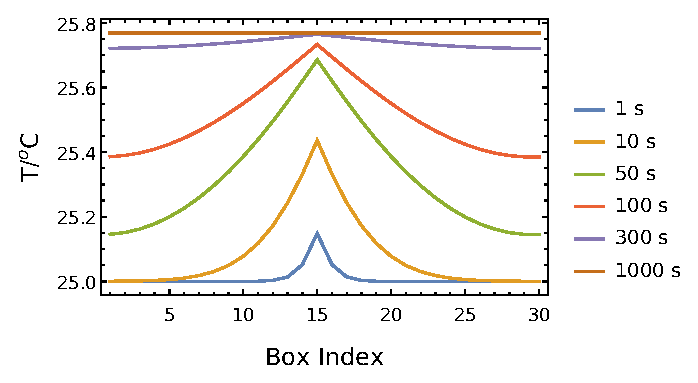
\includegraphics[width=0.37\textwidth]{figures/combustbox.eps}
\caption{Temperature curve over the whole box at different time. `0 s' stands for the `ignition'.}
\label{combustbox}
\end{figure}

Fig.\ref{diff} clarifies the change of heating speed over the whole simulation as well as experiment. An initial faster heating and subsequent slow one is identified in the figure, which is very reasonable w.r.t. the gradually reduced gradient of the temperature. This finding also indicates a better point of choice for the correction of temperature. The lines drawn are used to estimate the actual temperature of the initial state and the end state of the reaction, thus the point chosen should be as close as possible to the very beginning of the reaction. The trend of the increasing of temperature shows that the point where the heating speed reaches the highest is much closer, compared with the `median' point. 

\begin{figure}
\centering
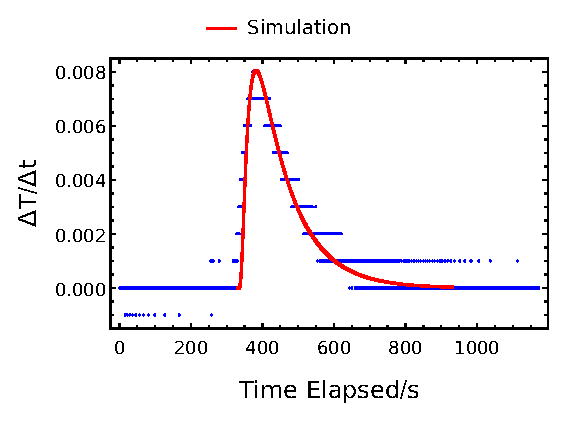
\includegraphics[width=0.35\textwidth]{figures/diff.eps}
\caption{$\frac{\Delta T}{\Delta t}$ curves for experiment and simulation}
\label{diff}
\end{figure}

\section{Conclusion}
The heat of combustion of stearyl alcohol is measured, whose result is relatively close to that in references. Simulations reveal the simplicity of the whole system, as well as indicating that the point where the heating speed reaches the highest better represents the time when the combustion occurs.

\bibliography{References}
\end{document}
